% =========================================================================
%  From Code to Theorem: The mistyR <-> Music of the Primes Bridge
%  Bridge-artifact series, 2026-07-12.
%  Companion to docs/motp-concordance.md (the maintained mapping) and
%  docs/motp-bridge-todo.md (the ledger). This PDF is the expository
%  snapshot: it EXPLAINS the connections the concordance only records.
% =========================================================================
\documentclass[11pt]{article}

\usepackage[margin=1.1in]{geometry}
\usepackage{amsmath, amssymb, amsthm}
\usepackage{booktabs}
\usepackage{array}
\usepackage{listings}
\usepackage{xcolor}
\usepackage{tikz}
\usetikzlibrary{positioning, arrows.meta}
\usepackage[colorlinks=true, linkcolor=blue!50!black, urlcolor=blue!50!black]{hyperref}
\usepackage{enumitem}

% -------------------------------------------------------------------------
% Book notation, reproduced locally.
% (We deliberately do NOT \input the book's preamble/commands.tex: it
% renews LaTeX built-ins (\and, \L, \P, \S, \d, \k, \a, \th) which is fine
% for the manuscript but hostile to any other document -- see ledger B16.
% Only the symbols this paper needs are defined, with safe names.)
% -------------------------------------------------------------------------
\newcommand{\MAlph}{\mathcal{L}}                 % musical alphabet L
\newcommand{\Lstar}{\MAlph^{*}}                  % note-letter space
\newcommand{\Lam}{\Lambda}                      % k-degree letter operator
\newcommand{\LSeq}{\mathbb{L}}                  % k-degree letter sequence
\newcommand{\Accset}{\mathcal{A}}               % accidental alphabet
\newcommand{\BL}{\overline{\textbf{Blk}}}       % black-supported letters
\newcommand{\WH}{\overline{\textbf{Wht}}}       % white letters
\newcommand{\DN}{\overline{\textbf{Den}}}       % den keys
\newcommand{\WN}{\overline{\textbf{WhtNeb}}}    % white neighbours
\newcommand{\Maj}{\Delta}                       % major quality
\newcommand{\Min}{\nabla}                       % minor quality
\newcommand{\FC}{\mathcal{F}}                   % furry-cat chain
\newcommand{\dist}{\tilde{d}}                   % degree-aware distance
\newcommand{\Zseven}{\mathbb{Z}_7}
\newcommand{\Ztwelve}{\mathbb{Z}_{12}}
\newcommand{\Freq}{\operatorname{Freq}}
\newcommand{\Colorf}{\operatorname{Color}}
\newcommand{\Accf}{\operatorname{Acc}}
\newcommand{\Letterf}{\operatorname{Letter}}
\newcommand{\pit}{\pi}                          % pitch label
\newcommand{\kernflat}{\texttt{-}}              % kern flat symbol

% -------------------------------------------------------------------------
% Theorem-ish environments. "Book" environments quote MOTP Chapter 2;
% "Bridge" environments are observations original to this paper.
% -------------------------------------------------------------------------
\theoremstyle{definition}
\newtheorem{bookdef}{Book Definition}[section]
\newtheorem{bookdist}[bookdef]{Book Distance Rule}
\newtheorem{bookthm}[bookdef]{Book Theorem}
\theoremstyle{remark}
\newtheorem{bridge}{Bridge Observation}[section]

% -------------------------------------------------------------------------
% R listings
% -------------------------------------------------------------------------
\definecolor{codebg}{RGB}{246,246,244}
\definecolor{codecomment}{RGB}{110,110,110}
\definecolor{codekw}{RGB}{25,60,130}
\lstset{
  language=R,
  basicstyle=\ttfamily\small,
  keywordstyle=\color{codekw},
  commentstyle=\color{codecomment}\itshape,
  backgroundcolor=\color{codebg},
  frame=single, framerule=0pt,
  xleftmargin=6pt, xrightmargin=6pt,
  breaklines=true,
  showstringspaces=false,
  columns=fullflexible,
  keepspaces=true
}

\newcommand{\code}[1]{\texttt{#1}}
\newcommand{\file}[1]{\texttt{#1}}

\title{\textbf{From Code to Theorem}\\[4pt]
\Large The \code{mistyR} $\longleftrightarrow$ \emph{Music of the Primes} Bridge}
\author{Ali Taqi\thanks{Prepared 2026-07-12 as part of the bridge-artifact series
(with Claude). Companion artifacts: \file{docs/motp-concordance.md} (the maintained
mapping) and \file{docs/motp-bridge-todo.md} (the ledger). This PDF is the
expository snapshot of the 2026-07-10 cross-reference audit.}}
\date{July 12, 2026}

\begin{document}
\maketitle

\begin{abstract}
\noindent
\code{mistyR} (2022) is an R implementation of Musical Set Theory: a core library
for spelling notes, intervals, and scales, plus two score-import modules
(\code{kern}, MIDI) feeding a stylometry suite. \emph{Music of the Primes} (MOTP,
2026) is a book manuscript whose Chapter~2, \emph{Chromatic-Accidental Arithmetic},
develops the same theory formally: a musical alphabet $\MAlph \cong \Zseven$, an
accidental norm $|\alpha|$, a family of white-key distance rules
$d_2, d_3, d_5, d_n$, and a transposition-invariance theorem. This paper explains,
construct by construct, how the two artifacts are the same mathematics written
twice --- once as executable R, once as definitions and theorems --- and documents
the places where each side outruns the other. The direction of the arrow matters:
the code came first, and the book is its \emph{retroactive formalization}. We give
the evidence (shared vocabulary fossils, identical algorithmic structure, a
theorem that is precisely a function's correctness argument), derive the central
identity \code{.WKsemitones} $\equiv d_n$, and map the full pipeline from
Chapter~2's arithmetic up through the modality stylometry that runs on real scores.
\end{abstract}

\tableofcontents
\newpage

% =========================================================================
\section{Introduction: Two Artifacts, One Theory}
% =========================================================================

Between 2022 and 2026, the same body of musical mathematics was written down twice.

The first time, it was written as software. \code{mistyR} is an R package that
spells scales in any key, computes scale degrees of arbitrary notes against
arbitrary tonics, resolves enharmonics, and parses \code{.krn} and \code{.mid}
scores into a shared tidy ``piece frame'' on which a suite of stylometric analyses
runs. Its core library (\file{R/}) is small --- six files --- and every function
in it encodes a fact about how Western pitch notation works.

The second time, it was written as mathematics. Chapter~2 of \emph{Music of the
Primes}, \emph{Chromatic-Accidental Arithmetic}, builds the same machinery from
first principles: the musical alphabet as $\Zseven$, accidentals as a signed norm,
step distances decided by the black-key layout of the piano, and a preservation
theorem that reduces all chromatic spelling problems to white-key problems.

Neither artifact cites the other, but they did not arise independently: the book
is the code's \emph{retroactive formalization}. The evidence is threefold, and
this paper is organized around it:

\begin{enumerate}[leftmargin=2em]
  \item \textbf{Identical algorithmic skeletons} (\S\ref{sec:distances}--\S\ref{sec:preservation}).
        The book's $n$-degree distance rule and the code's
        \code{.WKsemitones()} are the same computation; the book's
        Accidental-Transpositional Preservation Principle is, line for line, the
        correctness argument of the code's \code{scale()} function.
  \item \textbf{Vocabulary fossils} (\S\ref{sec:fossils}). The code's original,
        idiosyncratic word for accidentals --- \emph{incidental} --- survives
        inside two of the book's formal definitions. The code's ASCII workaround
        for double-sharps (\code{x}) fossilized into the book's typography.
  \item \textbf{Matched asymmetries} (\S\ref{sec:harmony}, \S\ref{sec:asymmetries}).
        Where the book has theory the code lacks (quality dyads/triads), there is
        \emph{no} implementation anywhere in the repository --- because that
        section is new mathematics, not formalization. Where the code has
        machinery the book lacks (double accidentals, enharmonic simplification,
        score parsing), the book's scope simply has not caught up.
\end{enumerate}

\paragraph{How to read this paper.} Each section takes one theoretical construct,
quotes the book's formulation, exhibits the code that implements it, and explains
the correspondence --- including, where they exist, the small divergences of
convention that make the mapping non-obvious at first sight. Book results are
quoted in \emph{Book Definition / Distance Rule / Theorem} environments, keyed by
their titles in \file{chapters/chapter2.tex} (never by page number, so the mapping
survives edits). Original observations are set as \emph{Bridge Observations}.
Appendix~\ref{app:translation} collects the entire translation key in one table.

\paragraph{The two repositories.}
\begin{center}
\renewcommand{\arraystretch}{1.25}
\begin{tabular}{@{}lll@{}}
\toprule
 & \textbf{Book} & \textbf{Code} \\
\midrule
Location & \file{music-of-the-primes/} & \file{mistyR/} \\
Scope here & Ch.~2 \emph{Chromatic-Accidental Arithmetic} & \file{R/} core; modules where noted \\
Objects & $\MAlph$, $\Lam_k$, $|\alpha|$, $d_n$, $\BL$, $\Maj/\Min$, $\FC$ & \file{data.R}, \file{accidental.R}, \file{interval.R}, \\
 & & \file{scale.R}, \file{harmony.R}, \file{analysis.R} \\
Born & 2026 (manuscript, active) & 2022 (prototype, revived 2026) \\
\bottomrule
\end{tabular}
\end{center}

% =========================================================================
\section{The Musical Alphabet: $\MAlph \cong \Zseven$}
% =========================================================================

\begin{bookdef}[Musical Alphabet]
The musical alphabet is a set of letters $\MAlph = \{A, B, \dots, F, G\}$, where
the letter after $G$ loops back to $A$. The book immediately notes
$\MAlph \cong \Zseven$: fixing $A = 0, B = 1, \dots, G = 6$, looping is addition
in the group of integers modulo $7$.
\end{bookdef}

The code declares the same object as a global in \file{data.R}:

\begin{lstlisting}
MUS_ALPH <- LETTERS[1:7]          # A B C D E F G
mod7 <- function(x) { x %% 7 }    # arithmetic modulo 7
note_index <- function(note){ which(MUS_ALPH == note) }
\end{lstlisting}

The isomorphism is realized by \code{note\_index()} --- except for one
convention divergence that echoes through the entire codebase:

\begin{bridge}[The off-by-one dance]\label{obs:offbyone}
The book works in $\Zseven = \{0,\dots,6\}$ with $A = 0$. R is 1-indexed, so the
code stores $A = 1, \dots, G = 7$ and must conjugate every modular operation
through the shift $x \mapsto x - 1$:
\begin{lstlisting}
.ALPH_RANGE <- function(i, length){    # wrapped range of letters
  range <- i:(i + (length - 1))
  range <- mod7(range - 1)             # shift down, reduce mod 7,
  range + 1                            # shift back up
}
.IDX_STATIC <- function(range){ mod7(range - 1) + 1 }
\end{lstlisting}
The recurring pattern $\code{mod7}(x-1)+1$ is the 1-indexed shadow of the book's
clean $\Zseven$ arithmetic. Reading the book as ``the version of the code where
the indexing finally got cleaned up'' is historically accurate: the formalization
chose $0$-indexing precisely because the prototype's $1$-indexed gymnastics were
noise.
\end{bridge}

% =========================================================================
\section{Letter Degrees and Sequences}\label{sec:degrees}
% =========================================================================

\begin{bookdef}[$k$-Degree Letter; $k$-Degree Letter Sequence]
For $L \in \MAlph$, the $k^{\text{th}}$ degree letter is
$\Lam_k(L) = L \oplus (k-1)$, the terminus of the sequence
$$\LSeq_k[L] = \{L,\; L \oplus 1,\; \dots,\; L \oplus (k-1)\},$$
where $\oplus$ is letter addition \emph{with looping}. The sequence has $k$
letters including the start, matching the musician's 1-indexed convention:
the ``fifth of $F$'' is $\Lam_5(F) = C$, reached after four steps.
\end{bookdef}

The code implements the operator and the sequence separately, in
\file{scale.R} and \file{data.R}:

\begin{lstlisting}
`%STEPUP%` <- function(scale, note){       # one application of L (+) 1
  idx <- note_index(note)
  scale[mod7(7 + idx) + 1]
}
`%STEP+%` <- function(note, steps){        # Lambda_k: iterate k-1 times
  for(i in 1:steps){ note <- MUS_ALPH %STEPUP% note }
  note
}
# The sequence L_k[L] is a wrapped index range:
# MUS_ALPH[.ALPH_RANGE(note_index(L), k)]
\end{lstlisting}

So $\Lam_k(L)$ = \code{L \%STEP+\% (k - 1)} and
$\LSeq_k[L]$ = \code{MUS\_ALPH[.ALPH\_RANGE(note\_index(L), k)]}. Both sides
share the same 1-indexed \emph{musical}-degree convention ($k$ letters, $k-1$
steps) even though the book's underlying letter arithmetic is 0-indexed --- the
$(k-1)$ in the book's definition is exactly the \code{degree\_n - 1} that appears
wherever the code builds intervals:

\begin{lstlisting}
# from .intervalNote() in interval.R:
white <- tonic %STEP+% (degree_n - 1)   # Lambda_k(tonic) = tonic (+) (k-1)
\end{lstlisting}

\begin{bridge}[Rule of 9 is book-only]
The book proves $\Lam_k(L) = L' \iff \Lam_{9-k}(L') = L$ (fifths pair with
fourths, sixths with thirds, sevenths with seconds). The code never inverts an
interval --- it always computes degrees directly --- so this theorem has no code
counterpart. It is one of the first places the formalization \emph{adds}
structure rather than transcribing it (see \S\ref{sec:asymmetries}).
\end{bridge}

The heptatonic scale template $\mathcal{S}_7[L] = \LSeq_7[L]$ (``the musical
alphabet, beginning at $L$'') is the code's \code{.baseScale()}
(\file{harmony.R}):

\begin{lstlisting}
.baseScale <- function(tonic){
  MUS_ALPH[.ALPH_RANGE(note_index(tonic), length = 7)]
}
\end{lstlisting}

% =========================================================================
\section{Pitch Labels and Accidental Arithmetic}\label{sec:accidentals}
% =========================================================================

\begin{bookdef}[Note-Letter; Accidentals]
An accidental is $\alpha \in \Accset = \{\flat, \natural, \sharp\}$. A pitch
label (note-letter) pairs a letter with an accidental:
$\pit = (L, \alpha) = L^{\alpha} \in \Lstar = \MAlph \times \Accset$. Flats and
sharps neutralize: $(L^{\flat})^{\sharp} = L^{\natural} = (L^{\sharp})^{\flat}$.
\end{bookdef}

In the code, a pitch label is simply a string (\code{"F\#"}, \code{"B-"}), and
the pair structure is recovered by two projections in \file{accidental.R}:

\begin{lstlisting}
.dropAccidental   <- function(note){ substring(note, 1, 1) }  # Letter(pi)
.detectAccidental <- function(note){ ... }                    # Acc(pi), via ACC_HASH
\end{lstlisting}

These are exactly the book's getters $\Letterf(\pit)$ and $\Accf(\pit)$ (macros
\code{\textbackslash Let}, \code{\textbackslash Acc} in
\file{preamble/commands.tex}). Applying an accidental --- the book's
$\pit \odot \alpha$ --- is the infix \code{\%ACC\%} wrapping
\code{.addAccidental()}, and the neutralization axiom is literally a branch of
that function:

\begin{lstlisting}
.addAccidental <- function(note, accidental){
  ...
  if(accidental == "flat"){
    if(note_acc == "flat")         { accidental <- "&" }  # bb (double flat)
    else if(note_acc == "natural") { accidental <- "b" }
    else if(note_acc == "sharp")   { accidental <- ""  }  # neutralization!
  }
  ...
}
\end{lstlisting}

\begin{bookdist}[Semitonal-Accidental Norm]
$d_{\alpha} : \MAlph \times \Lstar \to \{-1, 0, 1\}$ measures the distance between
a fixed letter and an accidentalized copy of itself:
$d_{\alpha}(L, L^{\alpha}) = |\alpha|$ where
$|\flat| = -1$, $|\natural| = 0$, $|\sharp| = +1$.
\end{bookdist}

The code's version is \code{.accidentalSemitones()} --- and here the code
\emph{extends} the book:

\begin{lstlisting}
.accidentalSemitones <- function(x, inverse = T){
  ACCIDENTAL <- c("&", "-", "", "#", "x")
  VALUE      <- c(-2,  -1,  0,  1,   2)
  if(inverse) { return(ACCIDENTAL[which(VALUE == x)]) }
  VALUE[which(ACCIDENTAL == x)]
}
\end{lstlisting}

\begin{bridge}[The norm, extended to doubles]\label{obs:doubles}
The code treats double accidentals as first-class citizens: the norm runs over
$\{-2, \dots, +2\}$ with symbols \code{\&} (double flat) and \code{x}
(double sharp), and the function is invertible in both directions --- it is used
\emph{norm-inverse-first} throughout the spelling engine (given a semitone
discrepancy, produce the accidental). The book's
$\Accset = \{\flat, \natural, \sharp\}$ truncates to singles even though
$\flat\flat$ and $\sharp\sharp$ appear in its own accidental-family tables ---
extending the Semitonal-Accidental Norm to $\pm 2$ is a pending book-side item
(ledger B14). This is the cleanest example of the code being \emph{ahead} of its
own formalization.
\end{bridge}

Note also the flat symbol: the code's canonical flat is the kern convention
\kernflat{} (so $B\flat$ is \code{"B-"}), with letter \code{b} accepted on input.
The book writes $\flat$ only. This single divergence explains most of the
surface-level unfamiliarity when reading one artifact with the other's eyes.

% =========================================================================
\section{Color: Black, White, and Den}\label{sec:color}
% =========================================================================

\begin{bookdef}[Black Flat-/Sharp-Supported Letters]
$L \in \BL[\flat] \iff \Colorf(L^{\flat}) = \mathbf{Blk}$, giving
$\BL[\flat] = \{A, B, D, E, G\}$ with complement $\WH[\flat] = \{C, F\}$.
Dually, $\BL[\sharp] = \{A, C, D, F, G\}$ with complement
$\WH[\sharp] = \{B, E\}$.
\end{bookdef}

This is a two-column boolean table in \file{data.R} --- arguably the single most
load-bearing data structure in the package:

\begin{lstlisting}
ALPH_HASH <- function(){
  MUS_ALPH <- LETTERS[1:7]                #  A B C D E F G
  HAS_FL <- as.logical(c(1,1,0,1,1,0,1))  #  Blk[flat]:  A B . D E . G
  HAS_SH <- as.logical(c(1,0,1,1,0,1,1))  #  Blk[sharp]: A . C D . F G
  data.frame(LETTER = MUS_ALPH, HAS_FL, HAS_SH)
}
\end{lstlisting}

The predicate $\Colorf$ is implemented directly:

\begin{lstlisting}
.isBlackNote <- function(note){
  note_acc    <- .detectAccidental(note)
  note_letter <- .dropAccidental(note)
  if(note_acc == "flat") { return(note_letter %in% HAS_FLATS)  }
  else if(note_acc == "sharp"){ return(note_letter %in% HAS_SHARPS) }
  FALSE
}
\end{lstlisting}

\begin{bridge}[Den keys are a book-native abstraction]
The book goes one step further and intersects the two supports:
$$\DN = \BL[\flat] \cap \BL[\sharp] = \{A, D, G\}
\quad (\text{mnemonic: ``A Den `G'\,''}),$$
with complement the \emph{white neighbours} $\WN = \{B, C, E, F\}$. The code
stores \code{HAS\_FL} and \code{HAS\_SH} but \emph{never intersects them} ---
no function computes or uses $\DN$. The den/neighbour classification is the
formalization discovering structure the prototype had in its data but never
named. (Adding \code{DEN\_KEYS} and \code{WHITE\_NEIGHBOURS} globals is ledger
A8 --- cheap, and it would let code comments cite the book.)
\end{bridge}

% =========================================================================
\section{Distance Rules and the White-Key Engine}\label{sec:distances}
% =========================================================================

This section contains the strongest single piece of evidence that book and code
are one theory. We first quote the book's two rules, then show they compose into
exactly the code's \code{.WKsemitones()}.

\begin{bookdist}[Step Distance]\label{rule:step}
$d_2 : \MAlph \to \{1, 2\}$ gives the semitone distance from a letter to its
right neighbour $\Lam_2 = L \oplus 1$:
$$d_2(L) =
  \begin{cases}
    1, & \Lam_2 \in \WH[\flat] \\
    2, & \Lam_2 \in \BL[\flat]
  \end{cases}
\qquad\text{equivalently}\qquad
d_2(L) =
  \begin{cases}
    1, & L \in \WH[\sharp] \\
    2, & L \in \BL[\sharp].
  \end{cases}$$
\end{bookdist}

\begin{bookdist}[$n$-Degree Distance]\label{rule:ndeg}
For $L \in \MAlph$ with $n^{\text{th}}$-degree letter $\Lam_n = L \oplus (n-1)$,
the distance accumulates step by step:
$$d_n(L) = d(L, \Lam_n) = \sum_{j} d_2(\Lam_j) = \sum_{j} d(\Lam_j, \Lam_{j+1}),$$
the sum running over the $n - 1$ steps from $L$ to $\Lam_n$.\footnote{The book's
display writes the summation bounds as $j = 0$ to $n-1$, which would take $n$
steps; since $\Lam_n = L \oplus (n-1)$, the intended count is $n-1$ steps
($j = 0$ to $n-2$). The code resolves the wobble unambiguously --- it counts
\code{degree - 1} steps --- and the book-side cleanup is part of the
distance-family naming item, ledger B7.}
\end{bookdist}

Now the code, from \file{interval.R}, verbatim:

\begin{lstlisting}
# Find the white-key range number of semitones between
# a note and a given scale degree
.WKsemitones <- function(note, degree){
  note_idx     <- note_index(note)
  range        <- .ALPH_RANGE(note_idx, degree)
  letter_range <- ALPHABET[range,]
  # Get the number of flats in range
  FLATS  <- sum(letter_range[2:degree,]$HAS_FL)
  # Get the number of white keys in the range (exclude tonic)
  WHITES <- degree - 1
  semitones <- FLATS + WHITES
  semitones
}
\end{lstlisting}

\begin{bridge}[The central identity: \code{.WKsemitones} $\equiv d_n$]
\label{obs:central}
Write the letters from $L$ to its $n^{\text{th}}$ degree as
$\Lam_0 = L, \Lam_1, \dots, \Lam_{n-1} = \Lam_n(L)$. By the Step Distance rule
(flat-side criterion), each step contributes
$$d_2(\Lam_j) = 1 + \big[\Lam_{j+1} \in \BL[\flat]\big],$$
i.e.\ one semitone always, plus one more exactly when the \emph{arrival} letter
is flat-supported. Summing the $n-1$ steps:
$$d_n(L) \;=\; \underbrace{(n-1)}_{\text{one per step}}
\;+\; \underbrace{\#\{\, j \in \{1,\dots,n-1\} : \Lam_j \in \BL[\flat] \,\}}_{\text{flat-supported arrivals}}.$$
The code computes precisely these two terms:
\code{WHITES = degree - 1} is the first, and
\code{FLATS = sum(letter\_range[2:degree,]\$HAS\_FL)} --- the count of
flat-supported letters in the range \emph{excluding the tonic}, i.e.\ among the
arrival letters $\Lam_1, \dots, \Lam_{n-1}$ --- is the second. The function is
the theorem; \code{HAS\_FL} is $\BL[\flat]$; the exclusion of row 1 is the
exclusion of $\Lam_0$ from the arrival set.

Note which criterion the code chose: the \emph{flat-side} case of
Rule~\ref{rule:step} only. The book's dual sharp-side formulation
($d_2(L) = 2 \iff L \in \BL[\sharp]$) appears nowhere in the code --- it is
added symmetry, discovered at formalization time.
\end{bridge}

The specialized rules are then corollaries on both sides. The book defines the
skip distance $d_3 : \MAlph \to \{3, 4\}$ (two steps; range constrained because
no two consecutive letters lie in $\WH[\flat] = \{C, F\}$ --- ``we cannot find 3
consecutive white keys on a piano'') and the triadic distance
$d_5 : \MAlph \times \MAlph \to \{6, 7\}$ (two skips; only diminished and perfect
fifths occur between white keys). The code never defines $d_3$ or $d_5$
separately --- it gets them for free as \code{.WKsemitones(note, 3)} and
\code{.WKsemitones(note, 5)}, exactly as the book gets them as instances of
$d_n$.

\begin{center}
\renewcommand{\arraystretch}{1.3}
\begin{tabular}{@{}llll@{}}
\toprule
\textbf{Book rule} & \textbf{Type} & \textbf{Range} & \textbf{Code realization} \\
\midrule
$d_2$ (Step) & $\MAlph \to \{1,2\}$ & step & \code{.WKsemitones(L, 2)} \\
$d_3$ (Skip) & $\MAlph \to \{3,4\}$ & third & \code{.WKsemitones(L, 3)} \\
$d_5$ (Triadic) & $\MAlph^2 \to \{6,7\}$ & fifth & \code{.WKsemitones(L, 5)} \\
$d_n$ ($n$-Degree) & $\MAlph^2 \to \Ztwelve$ & any & \code{.WKsemitones(L, n)} \\
$d_{\alpha}$ (Accidental Norm) & $\MAlph \times \Lstar \to \{-1,0,1\}$ & vertical & \code{.accidentalSemitones()} ($\pm 2$) \\
$d_{\square}$ (Octave) & $12k$ & octaves & (not needed; octave-free note space) \\
\bottomrule
\end{tabular}
\end{center}

% =========================================================================
\section{The Chromatic Algorithm: Spelling Any Interval}\label{sec:chromatic}
% =========================================================================

The book's ``Chromatic Algorithm'' --- described, memorably, as \emph{the
music-theory version of borrowing, like in 3rd-grade addition} --- spells an
arbitrary interval in two moves: lay down the white-key skeleton, then correct
with an accidental whose norm makes up the semitone difference. This is,
structurally and in order of operations, the code's \code{.intervalNote()}:

\begin{lstlisting}
.intervalNote <- function(tonic, degree){
  degree_n        <- parse_number(degree)
  semitones       <- SCALE_DEGREES[[degree]]        # target: q_k in Z12
  white           <- tonic %STEP+% (degree_n - 1)   # skeleton: Lambda_k
  semitones_white <- .WKsemitones(tonic, degree_n)  # skeleton's size: d_n
  accidental <- .accidentalSemitones(semitones - semitones_white)
  paste(white, accidental, sep = "")                # correction: |alpha|
}
\end{lstlisting}

Here \code{SCALE\_DEGREES} (\file{data.R}) is the book's interval table
$q_k \in \Ztwelve$ --- the map from degree labels to semitone counts
($\code{"1"} \mapsto 0$, $\code{"b3"} \mapsto 3$, $\code{"3"} \mapsto 4$,
$\code{"5"} \mapsto 7$, \dots).

\paragraph{Worked example (both notations).} Spell the major third of $D$.
\begin{itemize}[leftmargin=2em]
  \item \emph{Book:} the target is $q_{\text{M3}} = 4$ semitones. The skeleton is
        $\Lam_3(D) = F$, with $d_3(D) = d_2(D) + d_2(E) = 2 + 1 = 3$ (since
        $E \in \BL[\flat]$ but $F \in \WH[\flat]$). Borrow the difference:
        $4 - 3 = 1 = |\sharp|$, so the answer is $F^{\sharp}$.
  \item \emph{Code:} \code{SCALE\_DEGREES[["3"]]} $= 4$;
        \code{D \%STEP+\% 2} $=$ \code{"F"};
        \code{.WKsemitones("D", 3)} $= 1 + 2 = 3$ (one flat-supported arrival,
        $E$, plus two steps);
        \code{.accidentalSemitones(4 - 3)} $=$ \code{"\#"}; result \code{"F\#"}.
\end{itemize}
Same skeleton, same deficit, same correction --- and for the minor third
(\code{"b3"}, target 3) the deficit is $0$ and both sides answer $F^{\natural}$.

% =========================================================================
\section{The Preservation Principle is \code{scale()}'s Correctness Proof}
\label{sec:preservation}
% =========================================================================

\begin{bookthm}[Accidental-Transpositional Preservation Principle]
Let $L, L_* \in \MAlph$ be unaccidentalized letters with
$\dist(L, L_*) = k$ semitones, where $\dist$ is the degree-aware distance
(assuming the correct form $d_j$ for $L_* = \Lam_j(L)$). Fixing
$\alpha \in \Accset$ and accidentalizing \emph{both} letters by $\alpha$
preserves the distance:
$$\dist(L, L_*) = k \iff \dist(L^{\alpha}, L_*^{\alpha}) = k.$$
The book calls this a \emph{sufficiency result on the white keys}: every
spelling problem in $\Lstar$ reduces to one in $\MAlph$.
\end{bookthm}

Now read \code{scale()} (\file{scale.R}):

\begin{lstlisting}
scale <- function(tonic, scale_degrees){
  note_letter <- .dropAccidental(tonic)
  accidental  <- .detectAccidental(tonic)
  # (1) Solve the problem on the white keys
  base_scale <- .scaleBase(note_letter, scale_degrees)
  if(accidental == "natural"){ return(base_scale) }
  # (2) Transport the solution by the tonic's accidental
  purrr::map_chr(base_scale, .addAccidental, accidental)
}
\end{lstlisting}

\begin{bridge}[A theorem that is a function]\label{obs:thmfunction}
The function \emph{is} the theorem's proof strategy, executed:
strip the tonic's accidental (step into $\MAlph$), spell the entire scale on
white keys via the Chromatic Algorithm (\code{.scaleBase} maps
\code{.intervalNote} over the degree vector), then apply the tonic's accidental
to \emph{every} note of the result (transport back to $\Lstar$). The output is
correct \emph{if and only if} same-accidental transposition preserves all the
interval distances --- which is exactly what the Preservation Principle asserts.
The theorem is the correctness argument \code{scale()} always needed; the code
is the algorithmic content the theorem always had. So
\code{major\_scale("E-")} works by spelling the white-key $E$ major scale and
flattening all seven notes.
\end{bridge}

The same white-key-sufficiency reduction runs in the opposite direction in
\code{scaleDegree()} (\file{harmony.R}), which classifies an arbitrary note
against an arbitrary tonic. Rather than strip accidentals, it \emph{equalizes}
them --- sharpening flat tonics or flattening sharp tonics on both arguments
simultaneously, which is the Preservation Principle applied with
$\alpha^{-1}$ --- and then delegates to the white-key solver:

\begin{lstlisting}
else if(tonic_accidental == "flat" && (tonic_letter %in% HAS_FLATS)){
    tonic <- tonic %ACC% "#"; note <- note %ACC% "#"   # transpose BOTH up
    return(.scaleDegreeWK(tonic, note))                # solve on white keys
}
\end{lstlisting}

\begin{bridge}[The theorem as the spec for a known bug]\label{obs:complexcase}
The residual branch \code{.complexCase()} (tonics like $C^{\flat}$ or
$E^{\sharp}$, whose letter lacks the needed support) carries the confession
\emph{``doesn't quite do the trick; misses white keys...''} --- it reaches for
ad-hoc enharmonic cycling instead of same-accidental transposition, and the
degree information decays in transit. The clean fix is to apply the
Preservation Principle with the degree-aware $\dist$: reduce via
same-accidental transposition, never via enharmonics, so the letter-degree
skeleton survives. This is ledger item A6, and it is the purest example of the
book repaying its debt to the code: the 2026 theorem is the specification for
repairing the 2022 function.
\end{bridge}

% =========================================================================
\section{Furry Cats, Fifths, and the Key-Signature Table}\label{sec:furrycat}
% =========================================================================

\begin{bookthm}[Furry Cat Theorem]
The largest chain of fifths requiring no accidentals is unique: the white-key
sequence
$$\FC : F - C - G - D - A - E - B
\qquad (\text{``Furry Cats Get Dancey Around Every Bird''}),$$
with consecutive semitone distance $d(L_{i-1}, L_i) = 7 = \varphi$ throughout.
The chain terminates at $B$ because $d_5(B, F) = 6$: fixing it requires
$F \mapsto F^{\sharp}$, which breaks the next fifth and forces the chain
reaction that tiles the circle of fifths
$\FC^{\flat} - \FC^{\natural} - \FC^{\sharp}$.
\end{bookthm}

The code never states the theorem --- but it hard-codes its two consequences,
and their \emph{order of accrual}, in the key-signature table
(\file{data.R}, \code{.KEYS\_TABLE()}):

\begin{lstlisting}
key_sigs <- c("nosf",
  "f#","f#c#","f#c#g#","f#c#g#d#","f#c#g#d#a#",
  "f#c#g#d#a#e#","f#c#g#d#a#e#b#",            # sharps: F C G D A E B
  "b-e-a-d-g-c-f-","b-e-a-d-g-c-","b-e-a-d-g-",
  "b-e-a-d-","b-e-a-","b-e-","b-")            # flats:  B E A D G C F
\end{lstlisting}

Sharps accrue in exactly the furry-cat order $\FC$ (each new sharp is the next
cat), and flats accrue in the reversed chain $B\,E\,A\,D\,G\,C\,F$ --- the
book's circle of fourths $\mathcal{R}$. A musician memorizes these strings; the
theorem explains \emph{why} these and no others are the fifteen key signatures.
The book also derives the ``cursed shell spellings'' at the chain's seam ---
$\varphi(B^{\flat}) = F^{\natural}$, $\varphi(B^{\natural}) = F^{\sharp}$,
$\varphi(B^{\sharp}) = F^{\sharp\sharp}$ --- which is the single semitone gap
$d_5(B, F) = 6$ wearing three different accidentals.

% =========================================================================
\section{Enharmonics: Proper, Improper, and Simplification}\label{sec:enharmonics}
% =========================================================================

\begin{bookdef}[Chromatic Enharmonic]
The \emph{proper} enharmonic pairs are the two spellings of each black key:
$(A^{\sharp}, B^{\flat}), (C^{\sharp}, D^{\flat}), (D^{\sharp}, E^{\flat}),
(F^{\sharp}, G^{\flat}), (G^{\sharp}, A^{\flat})$. The white-key
(\emph{improper}) enharmonics are
$(B, C^{\flat}), (E, F^{\flat}), (B^{\sharp}, C), (E^{\sharp}, F)$.
\end{bookdef}

The code splits the definition into two operations along exactly the
proper/improper seam:

\begin{lstlisting}
# PROPER: cycle between a black key's two spellings
.cycle_enharmonic <- function(black_note){
  if(note_acc == "sharp"){ return((MUS_ALPH %STEPUP%   note_letter) %ACC% "b") }
  else if(note_acc == "flat"){ return((MUS_ALPH %STEPDOWN% note_letter) %ACC% "#") }
}
# IMPROPER: collapse a white-key spelling (Cb -> B, E# -> F, doubles too)
.simpler_enharmonic <- function(note){
  if(accidental == "flat" && !(note_letter %in% HAS_FLATS)){
    return( MUS_ALPH %STEPDOWN% note_letter )   # Cb -> B, Fb -> E
  }
  ...
}
\end{lstlisting}

The membership tests against \code{HAS\_FLATS} / \code{HAS\_SHARPS} are the
book's condition $\Colorf(L^{\alpha}) = \mathbf{Wht}$: a flat spelling is
improper precisely when the letter is not flat-supported. The shared word
\emph{improper} itself is part of the evidence --- see \S\ref{sec:fossils}.
Where the book's definition is a static list of pairs, the code additionally
makes simplification an \emph{operation} (including double-accidental cases
$F^{\flat\flat} \to E^{\flat}$), another instance of the implementation
outrunning the formalization.

% =========================================================================
\section{Tertiary Harmony: Where the Book Outruns the Code}\label{sec:harmony}
% =========================================================================

Chapter~2's \S\emph{Tertiary Harmony} develops a quality algebra: qualities
$\mathcal{Q} \in \{\Maj, \Min\}$ classify skips by size
($d_3 = 3 \Rightarrow \Min$, $d_3 = 4 \Rightarrow \Maj$); a \emph{quality dyad}
$\kappa_2 \mathcal{Q}[L^{\alpha}]$ assigns an accidental pair to a root and its
third; complementation satisfies the elegant
$$|\mathcal{Q}^c| = 7 - |\mathcal{Q}|
\qquad (3 + 4 = 4 + 3 = 7),$$
so a triad is a dyad stacked with its complement,
$\mathcal{Q}_3 = (L,\; \mathcal{Q}_2(L),\; \mathcal{Q}^c_2(T))$ --- every
white-key fifth splits as $\Min + \Maj$ or $\Maj + \Min$, and augmented chords
``are not naturally occurring'' between white keys.

\begin{bridge}[The one-way section]\label{obs:oneway}
\textbf{No chord constructor exists anywhere in mistyR.} The core library can
spell scales and classify degrees, but it cannot build a chord; the only
chord-adjacent code, \code{one\_chord\_harms()}
(\file{kern-module/R/kern-harmony.R}), \emph{extracts} simultaneities from
scores and diffs them mod 12:
\begin{lstlisting}
one_chord_harms <- function(chord){
  ...
  for(i in 2:l){ intervals[i-1] <- (chord[i] - chord[i-1]) %% 12 }
  intervals
}
\end{lstlisting}
That is analysis, not construction. \S\emph{Tertiary Harmony} is therefore the
one section of Chapter~2 that is \emph{new mathematics} rather than retroactive
formalization --- theory written for code that does not exist yet. The missing
implementation (a \code{dyad(L, quality)} / \code{triad(L, quality)} layer,
built on \code{\%ACC\%} and the $d_3$ classifier, which the library already
contains) is ledger item A9; landing it would make \S 2.3 retroactively true.
\end{bridge}

Fittingly, this is also where the strongest vocabulary fossil lives: both
Definition \emph{Quality Dyad} and Definition \emph{Quality Triad} describe
their accidental assignments as ``an assignment of an \textbf{incidental}
pair/triple'' --- the code's pre-2026 word surviving inside the book's most
code-independent section.

% =========================================================================
\section{Vocabulary Fossils: Evidence of Lineage}\label{sec:fossils}
% =========================================================================

Three shared idiosyncrasies establish the direction of the arrow beyond
reasonable doubt. None of them is standard music-theory or mathematical
usage; each originated as a quirk of the 2022 code and surfaced in the 2026
manuscript.

\begin{enumerate}[leftmargin=2em]
  \item \textbf{``Incidental.''} The code's original universal term for
        accidentals: \file{incidental.R}, \code{INC\_HASH}, \code{\%INC\%},
        \code{.addIncidental()}. The live code was renamed to the standard
        \emph{accidental} on 2026-07-10 (tag \code{pre-accidental-refactor}
        preserves the old vocabulary), but the book's Definitions
        \emph{Quality Dyad} and \emph{Quality Triad} still read ``an assignment
        of an \emph{incidental} pair $(\alpha, \alpha_T)$'' --- mistyR
        vocabulary fossilized inside the formalization.
  \item \textbf{``Improper.''} The code's \code{.improperStepDegree()}
        (\file{harmony.R}) handles tonic-letter-preserving alterations; the book
        classifies white-key enharmonics as \emph{improper enharmonics}
        (Definition \emph{Chromatic Enharmonic}). Same word, same seam of the
        same concept.
  \item \textbf{The bold x.} The code encodes double-sharp as ASCII \code{"x"}
        because \code{\#\#} confounded its regexes (the comment in
        \code{.ACC\_HASH\_EXT()} says so:
        \emph{``removed \code{\#\#} and \code{bb} due to regex confounding''}).
        The book writes the cursed-fifth spelling
        $\varphi(B^{\sharp}) = F^{\mathbf{x}}$ with a literal bold
        \code{x} --- even though \file{preamble/commands.tex} defines a proper
        $\sharp\sharp$ macro (\code{\textbackslash dsh}). An R regex workaround
        fossilized into the book's typography.\footnote{Fixed on the book side
        on 2026-07-10 (commit \code{400c574}): the display now uses
        \code{\textbackslash dsh}. The fossil is recorded here as history ---
        it was live evidence at audit time.}
\end{enumerate}

% =========================================================================
\section{From Theory to Stylometry: The Applied Layer}\label{sec:applied}
% =========================================================================

Everything above concerns the core library --- Chapter~2's mathematics. The
rest of the repository is what that mathematics is \emph{for}: reading real
scores and measuring their tonal style. This layer is outside Chapter~2's scope
(prospective material for later chapters), but it consumes the Chapter~2
machinery at every step, so the bridge extends naturally.

\subsection{The piece frame: one contract, two importers}

Both importers produce the same tidy frame --- piece columns
\code{key\_p}, \code{meter\_p}, \code{measure\_p}, plus one
(\code{rhythmN}, \code{note\_nameN}, \code{note\_valueN}) triplet per
simultaneous voice slot:

\begin{center}
\renewcommand{\arraystretch}{1.25}
\begin{tabular}{@{}lll@{}}
\toprule
 & \code{kern2df()} (\file{kern-module}) & \code{midi2df()} (\file{midi-module}) \\
\midrule
Source & \code{.krn} text splines & \code{.mid} binaries (via \code{tuneR}) \\
Simultaneity & spline columns & equal attack ticks, bass in slot 1 \\
Key & \code{*k[...]} signatures, windowed & Key Signature events, windowed \\
Spelling & as written in the score & key-aware per window (flat/sharp tables) \\
Since & 2022 (from Palmer's \code{museR}) & 2026 (parity importer, D2) \\
\bottomrule
\end{tabular}
\end{center}

Because the contract is shared, every analysis function runs on either format
unchanged --- a mixed kern+MIDI corpus is now a frame-level triviality.

\subsection{$\Ztwelve$ in the wild: note values}

The frame's \code{note\_value} column is the enharmonic collapse
$\Lstar \to \Ztwelve$ that Chapter~2 calls the semitone space --- implemented
as a 1-indexed scale rooted at $A^{\flat}$:
$$A^{\flat} = 1,\; A = 2,\; A^{\sharp} = B^{\flat} = 3,\; \dots,\; G = 12,\;
G^{\sharp} = 1 \;(\text{wrap}).$$
Proper enharmonics share values by construction (the book's ``twelve unique
notes, so there are enharmonic spellings''). The kern importer reads these off
a hash table (\code{KRN\_NOTE\_HASH}); the MIDI importer computes the same
scale from MIDI pitch classes by conjugating $\Ztwelve$ through the root shift:
\begin{lstlisting}
.m2df_note_value <- function(midi_note){ ((midi_note %% 12) + 4) %% 12 + 1 }
\end{lstlisting}
--- the same shift-conjugation pattern as Bridge Observation~\ref{obs:offbyone},
now aligning MIDI's $C$-rooted $\Ztwelve$ to misty's $A^{\flat}$-rooted
$\{1, \dots, 12\}$. And \code{one\_chord\_harms()} differencing consecutive
chord tones mod 12 is interval arithmetic in exactly this space.

\subsection{The stylometry chain runs on Chapter 2}

The modality features --- the repository's headline analysis --- are computed
per bar by classifying every note against the reigning tonic and counting
membership in hand-chosen scale-degree sets:

\begin{center}
\renewcommand{\arraystretch}{1.3}
\begin{tabular}{@{}lll@{}}
\toprule
\textbf{Feature} & \textbf{Major keys counts} & \textbf{Minor keys counts} \\
\midrule
\code{blues} & $\{\flat 3, \sharp 4, \flat 5, \flat 6\}$ & $\{3, \sharp 4, \flat 5\}$ \\
\code{interchange} & $\{\flat 3, \sharp 4, \flat 6, \flat 7\}$ & $\{\flat 2, 3, 6, 7\}$ \\
\code{borrowed\_sub} & $\{\flat 6, \sharp 5\}$ & $\{6\}$ \\
\code{consonance} & $\{1, 3, 5, 6\}$ & $\{1, \flat 3, 5, \flat 6\}$ \\
\code{dissonance} & \multicolumn{2}{l}{$\{\flat 2, \sharp 2, \sharp 4, \flat 5, \flat 7, 7\}$ (shared)} \\
\bottomrule
\end{tabular}
\end{center}

The degree labels those sets are matched against are \emph{produced by}
\code{scaleDegree()} --- the Preservation-Principle reduction of
\S\ref{sec:preservation} --- whose accidental prefixes come from
\code{.accidentalSemitones()}, the extended norm of \S\ref{sec:accidentals}.
The dependency chain, top to bottom:

\begin{center}
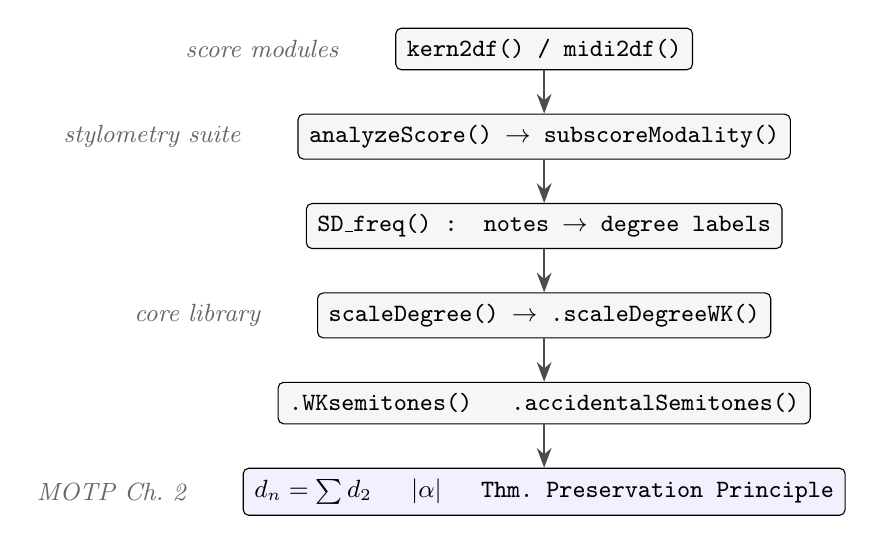
\begin{tikzpicture}[
  node distance=5.5mm and 8mm,
  box/.style={draw, rounded corners=2pt, fill=codebg, inner sep=4pt,
              font=\ttfamily\small, align=center},
  lab/.style={font=\itshape\small, text=black!60, align=right},
  arr/.style={-{Stealth[length=2.5mm]}, thick, black!70}
]
\node[box] (imp) {kern2df() / midi2df()};
\node[box, below=of imp] (ana) {analyzeScore() $\to$ subscoreModality()};
\node[box, below=of ana] (sdf) {SD\_freq() : notes $\to$ degree labels};
\node[box, below=of sdf] (sd)  {scaleDegree() $\to$ .scaleDegreeWK()};
\node[box, below=of sd]  (wk)  {.WKsemitones() \quad .accidentalSemitones()};
\node[box, below=of wk, fill=blue!6] (thy)
  {$d_n = \sum d_2$ \quad $|\alpha|$ \quad Thm.\ Preservation Principle};
\node[lab, left=6mm of imp] {score modules};
\node[lab, left=6mm of ana] {stylometry suite};
\node[lab, left=6mm of sd]  {core library};
\node[lab, left=6mm of thy] {MOTP Ch.\ 2};
\draw[arr] (imp) -- (ana);
\draw[arr] (ana) -- (sdf);
\draw[arr] (sdf) -- (sd);
\draw[arr] (sd)  -- (wk);
\draw[arr] (wk)  -- (thy);
\end{tikzpicture}
\end{center}

Every bluesiness score in \file{analysis/COMPOSERS.csv} is, at the bottom of
its call stack, an application of the $n$-degree distance rule and the
accidental norm. The applied layer is not adjacent to the theory --- it is
downstream of it.

Two further applied-layer constructs deserve book-side anchors when later
chapters arrive: \code{relative\_key()} (major-vs-relative-minor decided by a
tonic-and-fifth frequency vote --- an empirical procedure with no Chapter~2
analogue) and \code{DIATONIC\_SCALES} (the mode list --- Chapter~3's subject).

% =========================================================================
\section{Convention Divergences}\label{sec:divergences}
% =========================================================================

Five systematic differences of convention account for essentially all surface
friction when reading one artifact with the other's vocabulary. None is a
disagreement about content.

\begin{center}
\renewcommand{\arraystretch}{1.35}
\begin{tabular}{@{}p{3.4cm}p{4.6cm}p{4.6cm}@{}}
\toprule
\textbf{Axis} & \textbf{mistyR} & \textbf{MOTP} \\
\midrule
Letter indexing & 1-indexed (\code{LETTERS[1:7]}; the $\code{mod7}(x-1)+1$ dance) & 0-indexed $\Zseven$ ($A = 0$) \\
Degree operator & \code{\%STEP+\% (degree - 1)} & $\Lam_k = L \oplus (k - 1)$ \\
Flat symbol & kern \kernflat{} canonical; \code{b} accepted on input & $\flat$ only \\
Double accidentals & first-class: \code{\&}, \code{x}, norm $\pm 2$ & excluded from $\Accset$ (macros exist) \\
Step-distance criterion & flat-side only (\code{HAS\_FL}) & dual flat/sharp formulation \\
\bottomrule
\end{tabular}
\end{center}

One divergence is worth flagging as a live (mild) defect rather than a
convention: the code is internally inconsistent about which flat symbol it
\emph{emits} --- \code{enharmonic("F\#")} returns \code{"Gb"} (letter
\code{b}) while the spelling engine emits \code{"G-"} (kern), and only the
kern form round-trips through the score-analysis vocabulary
(\code{POSSIBLE\_NOTES}). Unifying on kern \kernflat{} is ledger A12.

% =========================================================================
\section{Asymmetries: What Each Side Has Alone}\label{sec:asymmetries}
% =========================================================================

\subsection*{Book-only (formalism beyond the code)}
\begin{itemize}[leftmargin=2em]
  \item \textbf{Den keys and white neighbours} ($\DN$, $\WN$) --- the
        intersection the code never takes (\S\ref{sec:color}).
  \item \textbf{Rule of 9} --- interval inversion pairing; the code never
        inverts (\S\ref{sec:degrees}).
  \item \textbf{Furry Cat Theorem as a stated result} --- the code hard-codes
        only its consequence, the key-signature table (\S\ref{sec:furrycat}).
  \item \textbf{The quality algebra} ($\Maj/\Min$ dyads, triads,
        complementation, stacking) --- no constructor exists
        (\S\ref{sec:harmony}).
  \item \textbf{The dual sharp-side step criterion} --- added symmetry
        (\S\ref{sec:distances}).
\end{itemize}

\subsection*{Code-only (implementation beyond the book)}
\begin{itemize}[leftmargin=2em]
  \item \textbf{Double accidentals as first-class} --- the norm extended to
        $\pm 2$ (\S\ref{sec:accidentals}; book remark pending, B14).
  \item \textbf{Enharmonic simplification as an operation} ---
        \code{.simpler\_enharmonic()}; the book only lists the pairs statically
        (\S\ref{sec:enharmonics}).
  \item \textbf{The entire applied layer} --- kern/MIDI parsing, the piece-frame
        contract, \code{relative\_key()} voting, and the modality/rhythm/harmony
        stylometry (\S\ref{sec:applied}); prospective material for later
        chapters.
\end{itemize}

The pattern in these lists is the thesis of this paper in miniature: the
book-only items are \emph{structure} (symmetries, dualities, named
abstractions, stated theorems) and the code-only items are \emph{machinery}
(edge cases, operations, I/O). That is precisely the signature of a
formalization written after --- and about --- a prototype.

% =========================================================================
\section{Maintenance and Companion Artifacts}\label{sec:maintenance}
% =========================================================================

This PDF is an expository \emph{snapshot}, dated 2026-07-12. The durable,
maintained mapping lives in two markdown companions inside the repository, and
the division of labor is deliberate:

\begin{itemize}[leftmargin=2em]
  \item \file{docs/motp-concordance.md} --- the mapping itself: translation
        key, fossils, asymmetries, divergences. Anchored to function names and
        definition titles (never line numbers) so it survives edits on both
        sides. \textbf{Update it when either side renames anything}; it is the
        artifact, its prose is secondary.
  \item \file{docs/motp-bridge-todo.md} --- the ledger: every insight that
        implies future work, with enough context to act on cold. Items cited in
        this paper: A6 (\code{.complexCase} via the Preservation Principle),
        A8 (den-key globals), A9 (dyad/triad constructors), A12 (flat-symbol
        unification), B7 (distance-family naming), B14 (double-accidental
        remark), D-track (module development).
  \item This paper (\file{docs/bridge-paper/}) --- the explanation: derivations,
        worked examples, and the argument for the direction of the arrow.
        Recompile after major renames; regenerate rather than patch if the
        theory itself moves.
\end{itemize}

When MOTP's other chapters gain code counterparts (Ch.~1 $\leftrightarrow$
tuning tables; Ch.~3 $\leftrightarrow$ \code{DIATONIC\_SCALES} and the mode
stylometry), extend the concordance chapter by chapter (ledger C1) and add
sections here rather than interleaving.

\appendix
% =========================================================================
\section{The Complete Translation Key}\label{app:translation}
% =========================================================================

The full symbol-to-construct mapping, in book order. (Maintained copy:
\file{docs/motp-concordance.md} \S1.)

\begin{center}
\renewcommand{\arraystretch}{1.4}
\small
\begin{tabular}{@{}p{4.1cm}p{4.1cm}p{5.2cm}@{}}
\toprule
\textbf{Book notation} & \textbf{Meaning} & \textbf{Code construct} \\
\midrule
$\MAlph = \{A, \dots, G\}$ & musical alphabet & \code{MUS\_ALPH} (\file{data.R}) \\
$\Zseven$, $\oplus$ (looping) & letter arithmetic mod 7 & \code{mod7()}, \code{.ALPH\_RANGE()}, \code{.IDX\_STATIC()} \\
$\Lam_k(L) = L \oplus (k-1)$ & $k$-degree letter & \code{\%STEP+\%}, \code{\%STEPUP\%} \\
$\LSeq_k[L]$ & $k$-degree letter sequence & \code{.ALPH\_RANGE(note\_index(L), k)} \\
$\mathcal{S}_7[L]$ & heptatonic template & \code{.baseScale()} (\file{harmony.R}) \\
$\pit = (L, \alpha) = L^{\alpha}$ & pitch label & note string (\code{"F\#"}, \code{"B-"}) \\
$\Letterf(\pit)$, $\Accf(\pit)$ & projections & \code{.dropAccidental()}, \code{.detectAccidental()} \\
$\pit \odot \alpha$ & apply accidental & \code{\%ACC\%} / \code{.addAccidental()} \\
$(L^{\sharp})^{\flat} = L$ & neutralization & the \code{""} branch of \code{.addAccidental()} \\
$|\alpha| \in \{-1, 0, 1\}$ & accidental norm & \code{.accidentalSemitones()} ($\pm 2$) \\
$\BL[\flat] = \{A,B,D,E,G\}$ & flat-supported letters & \code{HAS\_FL} / \code{HAS\_FLATS} \\
$\BL[\sharp] = \{A,C,D,F,G\}$ & sharp-supported letters & \code{HAS\_SH} / \code{HAS\_SHARPS} \\
$\Colorf(L^{\alpha})$ & key color & \code{.isBlackNote()} / \code{.isWhiteNote()} \\
$\DN = \{A, D, G\}$, $\WN$ & den keys, white neighbours & (none --- book-only; ledger A8) \\
proper / improper enharmonics & enharmonic pairs & \code{.cycle\_enharmonic()} / \code{.simpler\_enharmonic()} \\
$d_2$, $d_3$, $d_5$, $d_n$ & white-key distances & \code{.WKsemitones(note, degree)} \\
Chromatic Algorithm & skeleton $+$ borrowing & \code{.intervalNote()} \\
$q_k \in \Ztwelve$ & degree $\to$ semitones & \code{SCALE\_DEGREES} \\
Thm.\ Preservation Principle & transposition invariance & \code{scale()}'s structure; \code{scaleDegree()}'s reduction \\
$\FC$ (furry-cat chain) & chain of fifths & \code{.KEYS\_TABLE()} accrual order \\
$\Ztwelve$ collapse & enharmonic identification & \code{note\_value} ($A^{\flat} = 1$); \code{KRN\_NOTE\_HASH} \\
$\Maj / \Min$ dyads, triads & quality algebra & (none --- book-only; ledger A9) \\
Modes (Ch.~3) & diatonic modes & \code{DIATONIC\_SCALES} \\
\bottomrule
\end{tabular}
\end{center}

% =========================================================================
\section{Function Index}\label{app:functions}
% =========================================================================

Where to find each function cited in this paper, with its book anchor.

\begin{center}
\renewcommand{\arraystretch}{1.35}
\small
\begin{tabular}{@{}llp{5.6cm}@{}}
\toprule
\textbf{Function} & \textbf{File} & \textbf{Book anchor (Ch.~2 unless noted)} \\
\midrule
\code{mod7}, \code{note\_index}, \code{.ALPH\_RANGE} & \file{R/data.R} & Note $\MAlph \cong \Zseven$ \\
\code{ALPH\_HASH} (\code{HAS\_FL}/\code{HAS\_SH}) & \file{R/data.R} & Defs.\ Black Flat-/Sharp-Supported \\
\code{SCALE\_DEGREES} & \file{R/data.R} & interval table $q_k$ \\
\code{.KEYS\_TABLE} & \file{R/data.R} & Furry Cat Thm.\ (consequence) \\
\code{\%STEPUP\%}, \code{\%STEP+\%} & \file{R/scale.R} & Def.\ $k$-Degree Letter \\
\code{scale}, \code{.scaleBase} & \file{R/scale.R} & Thm.\ Preservation Principle \\
\code{diatonic\_scale}, \code{blues\_scale} & \file{R/scale.R} & (applications) \\
\code{\%ACC\%}, \code{.addAccidental} & \file{R/accidental.R} & $\pit \odot \alpha$; Note Accidental Neutralization \\
\code{.detectAccidental}, \code{.dropAccidental} & \file{R/accidental.R} & $\Accf$, $\Letterf$ \\
\code{.accidentalSemitones} & \file{R/accidental.R} & Distance Rule Semitonal-Accidental Norm \\
\code{.isBlackNote}, \code{.isWhiteNote} & \file{R/accidental.R} & $\Colorf$ \\
\code{enharmonic}, \code{.cycle\_enharmonic}, \code{.simpler\_enharmonic} & \file{R/accidental.R} & Def.\ Chromatic Enharmonic \\
\code{.intervalNote} & \file{R/interval.R} & Chromatic Algorithm \\
\code{.WKsemitones} & \file{R/interval.R} & Distance Rules Step / $n$-Degree \\
\code{scaleDegree}, \code{.scaleDegreeWK} & \file{R/harmony.R} & white-key sufficiency reduction \\
\code{.complexCase} & \file{R/harmony.R} & (known bug; theorem is the spec --- A6) \\
\code{.improperStepDegree} & \file{R/harmony.R} & improper enharmonics (vocabulary) \\
\code{.baseScale} & \file{R/harmony.R} & Def.\ Heptatonic Scale Template \\
\code{analyzeScore}, \code{subscoreModality}, \code{SD\_freq}, \code{modality} & \file{R/analysis.R} & (applied layer, \S\ref{sec:applied}) \\
\code{kern2df}, \code{relative\_key} & \file{kern-module/R/kern-import.R} & (applied layer) \\
\code{one\_chord\_harms}, \code{scale\_degree\_freq} & \file{kern-module/R/kern-harmony.R} & $\Ztwelve$ interval arithmetic \\
\code{rhythm\_freq}, \code{rhythm\_entropy}, \code{beat\_density} & \file{kern-module/R/kern-rhythm.R} & (applied layer) \\
\code{midi2df} and \code{.m2df\_*} helpers & \file{midi-module/R/midi-import.R} & (applied layer; parity importer) \\
\bottomrule
\end{tabular}
\end{center}

\end{document}
